%%%%%%%%%%%%%%%%%%%%%%%%%%%%%%%%%%%%%%%%%%%%%%%%%%%
%
%  New template code for TAMU Theses and Dissertations starting Fall 2016.  
%
%
%  Author: Sean Zachary Roberson
%  Version 3.17.09
%  Last Updated: 9/21/2017
%
%%%%%%%%%%%%%%%%%%%%%%%%%%%%%%%%%%%%%%%%%%%%%%%%%%%

%%%%%%%%%%%%%%%%%%%%%%%%%%%%%%%%%%%%%%%%%%%%%%%%%%%%%%%%%%%%%%%%%%%%%%%
%%%                           SECTION II
%%%%%%%%%%%%%%%%%%%%%%%%%%%%%%%%%%%%%%%%%%%%%%%%%%%%%%%%%%%%%%%%%%%%%%


\chapter{THEORETICAL FRAMEWORK}
\section{The Standard Model}
Particle physics is the study of the fundamental constituents of matter and the forces between them. For more than 40 years these have been described by the so-called standard model of particle physics (SM), which aims to provide, at least in principle, a basis for understanding all known particle interactions. The SM currently fails to include gravity due to the difficult task of combining the quantum theory used to describe the microscopic world and the general theory of relativity. Furthermore, its theorized force carrier, the graviton hasn't been found experimentally.

The SM can be understood as arising from an underlying symmetry of the universe, which combines the theory of electroweak (EW) interactions and that of quantum chromodynamics (QCD). In mathematical terms, the SM is formed from the gauge groups $SU(3)_{C}\times SU(2)_{L} \times U(1)_{EM}$. 

\section{Structure and Particle Content}
All the phenomena described by particle physics can be explained in terms of the properties and interactions of a small number of particles of four distinct types: two spin-1/2 families of fermions called leptons and quarks; one family of spin-1 bosons (called gauge bosons) which act as "force carriers", and a spin-0 particle, called the Higgs boson \cite{20121}, \cite{201230}. We should note that all particles in the SM are assumed to be elementary, i.e. they do not have internal structure or excited states.

In this section, the particle content of the SM will be introduced, along with the various force carriers. In the following sections, the specifics of particle-particle interactions will be explained in detail.

    \begin{figure}[h]
 	\centering
 	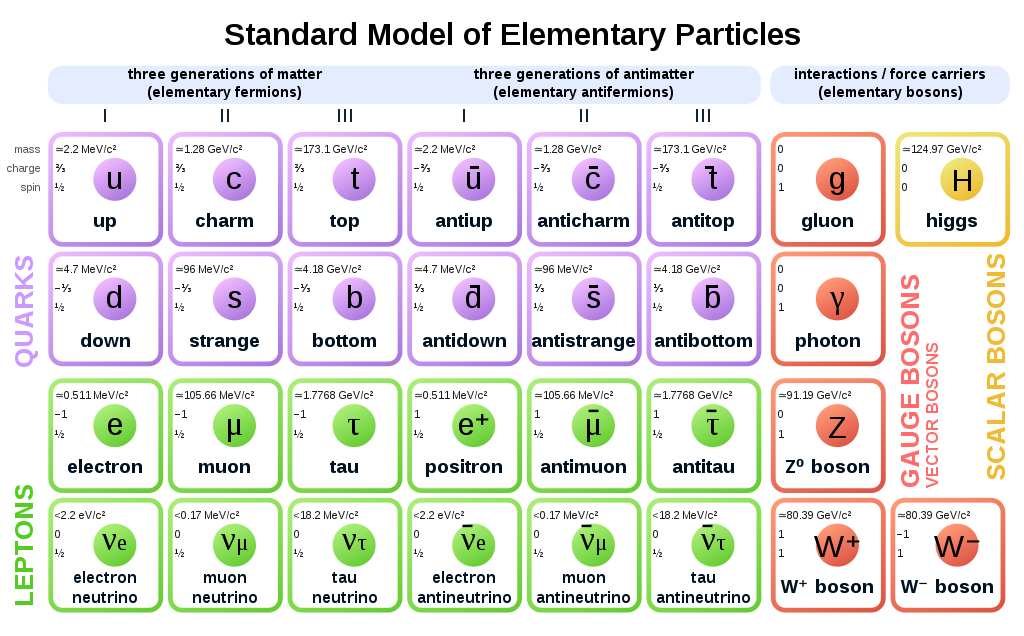
\includegraphics[width=0.75\textwidth]{figures/SMall.png}
 	\singlespace
 	\caption{Particles of the Standard Model of particle physics. Reprinted from \cite{StandardModelDiagram}}
 	\label{fig:stdmcer}
	\end{figure}

\subsection{Fermions}
Fermions are elementary particles with half-integer spin. They constitute the matter content of the SM, which accounts for 12 named fermions that interact via the weak and electromagnetic force (with the exception of neutrinos). Also, they obey Fermi-Dirac statistics and the Pauli exclusion principle, meaning that no two fermions can occupy the same quantum state within a quantum system simultaneously.

%The particle content of the SM can be divided into two additional categories of six fermions each, the quarks and the gluons. Quarks must bind together due to their strong force interaction, whereas the leptons can exist independently. Quarks are known to bind into triplets and doublets, called baryons and mesons, respectively.

%Moreover, fermions are grouped into 3 families or generations of 4 particles (2 quarks and 2 leptons), according to their masses. Each subsequent generation being a heavier version of the previous generation, with the same quantum numbers (neutrinos may have a different mass order). Therefore, the particle formed from Generation I particles are usually more stable and long-lived than those made from Generation III particles. Protons and neutrins themselves are made up of up and down quarks.

\subsubsection{Leptons}
There are six known leptons, and they occur in pairs called generations, which we can write as doublets:

\begin{equation}
	\begin{pmatrix}
		\nu_{e}\\
		e^{-}
	\end{pmatrix},
\begin{pmatrix}
		\nu_{\mu}\\
		\mu^{-}
	\end{pmatrix},
	\begin{pmatrix}
		\nu_{\tau}\\
		\tau^{-}
	\end{pmatrix}
\end{equation}

The three charged leptons ($e^{-}, \mu^{-},\tau^{-}$) all have electric charge $Q=-q$. Associated with them are three neutral leptons, or neutrinos, called the electron neutrino, mu neutrino, and tau neutrino, respectively, all of which have very small masses. The six distinct types of leptons are also referred to as having different "flavors". 

The charged leptons interact via both the electromagnetic and weak forces, whereas for neutral leptons only weak interactions have been observed. We should note that each generation of leptons has an associated quantum number. The electron number, which is defined for any state by

\begin{equation}
\label{lepn}
L_{e}\equiv N(e^{-}) - N(e^{+}) + N(\nu_{e}) - N(\bar{\nu_{e}}),
\end{equation}

where $N(e^{-})$ is the number of electrons present, and so on. For single-particle states, $L_{e} = 1$ for $e^{-}$ and $\nu_{e}$, $L_{e}=-1$ for $e^{+}$ and $\bar{\nu_{e}}$, and $L_{e}=0$ for all other particles.

The form of Equation \ref{lepn} also applies to the heavier lepton generations. Finally, in the SM, lepton numbers are individually conserved in all known interactions.

\subsubsection{Quarks}
Currently, there are six known quarks in the SM. Like the leptons, these six distinct types, or flavors, occur in pairs, or generations, denoted

\begin{equation}
	\begin{pmatrix}
		u\\
		d
	\end{pmatrix},
\begin{pmatrix}
		c\\
		s
	\end{pmatrix},
	\begin{pmatrix}
		t\\
		b.
	\end{pmatrix}
\end{equation}

Each generation consists of a quark with electromagnetic charge +2/3 ($u$,$c$, or $t$) together with a quark of charge -1/3 ($d$,$s$,$b$), in units of $q$. They are called the down($d$), up($u$), strange($s$), charmed($c$), bottom($b$) and top($t$) quarks. Each of these particles has an anti-particle version, with the same quantum numbers, but opposite charge. Furthermore, each quark also carries a \textit{color charge} which can be red, green, or blue. This is a result of the strong force interaction of the quarks and will be explained in more detail in Section \ref{strongint}.

%Although there is no evidence for the existence of free quarks, or any other fractionally charged particle, close to two hundred of their bound states have been discovered. All of them having integer electric charges. 
Quarks are known to bound to other quarks in states that we call hadrons. Hadrons can be bound states of two or three quarks called mesons and baryons, respectively. Recently, the LHCb collaboration reported the observation of a new type of hadron, a so-called \textit{pentaquark}, which is a bound state composed of four quarks and one anti-quark\cite{PhysRevLett.115.072001}.

%These bound states of quarks (hadrons) have several quantum numbers associated with them, referring to their quark content. For example, the \textit{strangeness} $S$ is defined by

%\begin{equation}
%S\equiv -N_{s}\equiv -[N(s)-N(\bar{s})]
%\end{equation}

%where $N(s)$ and $N(\bar{s})$ are the number of $s$ quarks and $\bar{s}$ antiquarks present in the state. Clearly, $S=-1$ for an $s$ quark, $S=1$ for an $\bar{s}$ antiquark and $S=0$ for all other quarks and antiquarks. The $up(U)$, $down(D)$, $charm (C)$, $bottom(B)$, and $top(T)$ quantum numbers are similarly defined.

%Furthermore, we can define a \textit{baryon number} $\tilde{B}$ of the state given by

%\begin{equation}
%\tilde{B} \equiv \frac{1}{3}[N(q)-N(\bar{q})]
%\end{equation}

%Baryon number $\tilde{B} = 1$ for baryons, $\tilde{b}=-1$ for antibaryons and $\tilde{B}=0$ for mesons.


\subsection{Bosons}
The SM bosons are the mediators of the interaction between the matter content of the SM, but also within themselves. They have integer spin quantum numbers and follow Bose-Einstein statistics, which means that they are not limited to single occupancy of the same quantum state. There are 6 named bosons: the gluon, the photon, the $W^{\pm}$, and the Z, which have spin 1; and the Higgs boson, which corresponds to a scalar field and therefore has spin 0.

\section{Particle Interactions}
The interactions of the particles described in the previous section can be described in the mathematical framework of gauge field theory. Three of the four fundamental forces of nature are described in the SM (electromagnetism, the strong and the weak force). To each of these forces belongs a physical theory, its corresponding charge, (i.e. electric charge, color or flavor) and an associated boson as mediator. 

Charges correspond to the time-invariant generators of a symmetry group, and specifically, to the generators that commute with the Hamiltonian. The invariance of the charge corresponds to the vanishing commutator

\begin{equation}
[Q, H] = 0
\end{equation}

for a given charge $Q$ and Hamiltonian $H$. Thus charges are associated with conserved quantum numbers; which are the eigenvalues $q$ of the generator $Q$ \cite{wiki:charge}. 

Modern theories describe these forces in terms of quantum fields, namely quantum electrodynamics (QED), QCD and the unified electroweak quantum field theory. One feature all these theories have in common is that they are all gauge invariant. This is important because it is a fundamental requirement from which the detailed properties of the interaction are deduced, as we shall see later in this section.

To describe each of the three SM interactions or forces, we will start with a Lagrangian that describes the general dynamics of a given system of particles. Then we will study its invariance(variance) under a global(local) gauge transformation. We will see that in order to maintain gauge invariance after a local transformation, we will need to introduce additional gauge fields and their corresponding covariant derivatives. Finally, we will take a look at the conservation laws arising from the symmetry of the gauge invariance \cite{Noether1918}.

\subsection{Quantum Electrodynamics}

QED describes the dynamics of the electromagnetic interaction between fermions and the boson mediating the interaction, the photon. QED corresponds to the $U_{EM}$ group and it was the first discovered example of gauge symmetry.% and it was developed from classical field theory.

In QFT, particles are represented by fields\cite{Peskin:1995ev}, which are in turn represented mathematically by Lagrangian densities $\mathcal{L}$. If we start with the Lagrangian density for the Dirac spin-1/2 fermion field\cite{wiki:diracfield}

\begin{equation}
\mathcal{L} = \bar{\psi}(i\gamma^{\mu}\partial_{\mu} - m)\psi
\end{equation}

where $\gamma^{\mu}$ are the gamma matrices\cite{wiki:gammam}, $\psi$ is a four-component column vector representing the wave function of a spin 1/2 particle (or Dirac spinor), $\bar{\psi}=\psi^{\dagger}\gamma^{0}$, and $m$ is the mass of the particle. The Lagrangian is invariant under a global U(1) transformation of the form

\begin{equation}
\label{gloTrans}
\psi \rightarrow \psi '= e^{-i\alpha}\psi
\end{equation}

while the parameter $\alpha$ is kept a constant. If instead, $\alpha$ is allowed to vary as a function of space-time, then Equation \ref{gloTrans} becomes a local U(1) transformation and the Lagrangian density becomes

\begin{equation}
\mathcal{L}\rightarrow \mathcal{L'} = \mathcal{L} + \bar{\psi}\gamma^{\mu}(\partial_{\mu}\alpha(x))\psi
\end{equation}

which is not invariant under the local transformation.

In order to restore local gauge invariance, a gauge field $A_{\mu}$ representing the photon and the covariant derivative 

\begin{equation}
D_{\mu} = \partial_{\mu} + iq A_{\mu}
\end{equation} 

, where $q$ (electric charge) are introduced. The new gauge field transforms as

\begin{equation}
A_{\mu}\rightarrow A'_{\mu} = A_{\mu} + \partial_{\mu}\chi(x)
\end{equation}

, where $\chi(x)$ is an arbitrary function of space-time. The covariant derivative has the same transformation properties as $\psi$ and is chosen to replace $\partial_{\mu}$.

After introducing these modifications, the Lagrangian takes the form:

\begin{equation}
\mathcal{L} = \bar{\psi}(i\gamma^{\mu}D_{\mu}-m)\psi - \frac{1}{4}F_{\mu\nu}F^{\mu\nu}
\end{equation}

where $F_{\mu\nu}= \partial_{\mu}A_{\nu} - \partial_{\nu}A_{\mu}$ is the electromagnetic field strength tensor. 

By looking at the resulting Lagrangian after the introduction of new gauge fields we can see that it does not include a mass term for the photon field (i.e. no term proportional to $~m^{2}A_{\mu}A^{\mu}$). At this point, the theory posits an infinite range for the interaction (which is experimentally verified).

The final form of the Lagrangian includes lepton-photon interactions, as well as those in the form of $l^{+}l^{-}\gamma$ and a quadratic term in the field strength tensor which is the photon kinetic energy. It can be generalized to include all the electromagnetically-charged fermions in the SM by taking the form

\begin{equation}
\mathcal{L} = \sum_{i}\bar{\psi_{i}}(i\gamma^{\mu}D_{\mu}-m_{i})\psi_{i} - \frac{1}{4}F_{\mu\nu}F^{\mu\nu}
\end{equation}

where $i=e,\mu,\tau,u,d,c,s,t,b$.

\subsection{Electroweak Interaction}

The story of weak interactions starts with Henri Becquerel's discovery of radioactivity in 1896 and its subsequent classification into alpha, beta and gamma decays of the nucleus by Ernest Rutherford and others. But the real understanding of beta-decay in the sense we now know it came only after Enrico Fermi formulated a physical mechanism for such process in 1934.

The main ingredient for Fermi's theory had been provided by Wolfgang Pauli. To solve the puzzle of the continuous energy spectrum of the electrons emitted in the beta-decay of the nuclei, Pauli had suggested that along with the electron, an almost massless neutral particle was also emitted. Fermi succeeded in incorporating Pauli's suggestion and thus was born the theory of weak interactions \cite{Rajasekaran:2014vza}.

In the 1960s Glashow, Salam, and Weinberg had developed a theory\cite{Glashow:1961tr,PhysRevLett.19.1264,salam} that unified electromagnetic and weak interactions in a way that is often compared to the unification of electric and magnetic interactions by Faraday and Maxwell a century earlier. This new theory made several remarkable predictions, including the existence of a neutral vector boson $Z^{0}$ and of weak reactions arising from its exchange.

The EW interaction is based on a local $SU(2)_{L}\times U(1)_{Y}$ gauge symmetry where $L$ and $Y$ are the generators of the symmetry. Here, electromagnetic and weak interactions are unified into a single non-abelian gauge theory. In order to understand this unification, we will start with a fermionic doublet representing an $SU(2)$ symmetry

\begin{equation}
\psi = \begin{pmatrix}
	\psi_{1}(x) \\
	\psi_{2}(x)
\end{pmatrix}, u_{R}, d_{R}
\end{equation}

which transforms under the three dimensional rotation

\begin{equation}
\psi\rightarrow exp<i\alpha^{i}\frac{\sigma_{i}}{2}>\psi
\end{equation}

which is the three dimensional version of Equation \ref{gloTrans} and $\sigma^{i}$ are the Pauli sigma matrices: the three non-commuting generators of the SU(2) transformations.

Just like in Section 2.3.1, we allow the parameter $\alpha$ to vary as a function of space-time so that

\begin{equation}
\psi(x)\rightarrow V(x)\psi(x)
\end{equation}
, where $V(x)= exp(i\alpha^{i}(x)\frac{\sigma^{i}}{2})$.

In order to keep the Lagrangian invariant under this transformation, we introduce additional fields. Since SU(2) has three generators there are also three gauge fields $A_{\mu}^{i}(x)$. The covariant derivative for a SU(2) gauge invariant Lagrangian is

\begin{equation}
\label{su2cod}
D_{\mu} = \partial_{\mu} - igA_{\mu}^{i}\frac{\sigma^{i}}{2}
\end{equation}

and therefore

\begin{equation}
A_{\mu}^{i}(x)\frac{\sigma^{i}}{2}\rightarrow V(x)(A_{\mu}^{i}(x)\frac{\sigma^{i}}{2}+\frac{i}{g}\partial_{\mu})V^{\dagger}(x)
\end{equation}

To simplify this calculation, we can expand $V(x)$ to first order in $\alpha$ 

\begin{equation}
A_{\mu}^{i}\frac{\sigma^{i}}{2}\rightarrow A_{\mu}^{i}\frac{\sigma^{i}}{2} + \frac{1}{g}(\partial_{\mu}\alpha^{i})\frac{\sigma^{i}}{2} + i[\alpha^{i}\frac{\sigma^{i}}{2}, A_{\mu}^{i}\frac{\sigma^{i}}{2}] + ...
\end{equation}

The covariant derivative will have the form

\begin{equation}
D_{\mu}\psi\rightarrow(1+i\alpha^{i}\frac{\sigma^{i}}{2})D_{\mu}\psi
\end{equation}

Due to the non-commutativity of the generators of this symmetry, the field strength tensor has an extra term

\begin{equation}
F_{\mu\nu}^{i} = \partial_{\mu}A_{\nu}^{i} - \partial_{\nu}A_{\mu}^{i} + g\epsilon^{ijk}A_{\mu}^{j}A_{\nu}^{k}
\end{equation}

We can the construct the Yang-Mills Lagrangian

\begin{equation}
\mathcal{L} = -\frac{1}{4}(F_{\mu\nu}^{i})^{2}+\bar{\psi}(i\gamma^{\mu}\partial_{\mu}-igA_{\mu}^{i}\frac{\sigma^{i}}{2})\psi
\end{equation}

Now we introduce the local gauge invariance requirement for the Lagrangian and introduce new gauge fields with their associated covariant derivatives.

But first, we should note that the SM fermions possess a fundamental property called chirality, which describes how a given particle's wave function behaves under rotation. In the SM, the left-handed components of the electron neutrino and electron are grouped into an SU(2) doublet. Since the right-handed component of the electron is invariant under SU(2), it is placed in a singlet, i.e.:

\begin{equation}
L_{e} = \begin{pmatrix}
	\nu_{e} \\
	e_{L}
\end{pmatrix}
, e_{R}
\end{equation}
 And so on for the heavier generations of leptons. 

Within the SM framework, neutrinos are weakly-interacting massless particles. As such, neutrinos wouldn't be able to change their handedness, but with mass, they can. Until \
now there is no experimental evidence for right handed neutrinos.

 The kinetic energy term of the electroweak Lagrangian for first generation leptons can be represented by:

 \begin{equation}
 \mathcal{L}_{KE}^{e} = L_{e}^{\dagger}\tilde{\sigma}^{\mu}i\partial_{\mu}L_{e}+ e_{R}^{\dagger}\sigma^{\mu}i\partial_{\mu}e_{R}
 \end{equation}
where $\sigma = (\sigma^{0}, \sigma^{1},\sigma^{2}, \sigma^{3})$, $\tilde{\sigma} = (\sigma^{0}, -\sigma^{1},-\sigma^{2}, -\sigma^{3})$, $\sigma^{0}$ is an identity matrix, and the $\sigma^{i}$ are again the Pauli matrices. This Lagrangian is invariant under the global $SU(2)_{L}\times U(1)_{Y}$ transformation:

\begin{equation}
L\rightarrow L' = e^{i\theta}UL\\
\end{equation}

\begin{equation}
e_{R}\rightarrow e'_{R} = e^{2i\theta}e_{R}
\end{equation}

where

\begin{equation}
U = e^{-ia^{k}\sigma^{k}}
\end{equation}

and $\theta$ and $a^{k}$ are real numbers parameterizing the transformation.

 Again, the Lagrangian is not invariant under a transformation where these parameters are allowed to vary as a function of space-time, i.e. a local transformation.

To restore invariance, we can introduce additional gauge fields and replace the space-time derivatives with an appropriately chosen covariant derivative. This time, we introduce a U(1) gauge field $B_{\mu}(x)$ and three SU(2) gauge fields $W_{\mu}(x)= W_{\mu}^{k}(x)\sigma_{k}$. Such fields must transform as

\begin{equation}
B_{\mu}(x)\rightarrow B'_{\mu}(x) = B_{\mu}(x) + \frac{2}{g_{1}}\partial_{\mu}\theta(x)
\end{equation}
\begin{equation}
W_{\mu}(x)\rightarrow W'_{\mu}(x) = U(x)W_{\mu}(x)U^{\dagger}(x) + \frac{2i}{g_{2}}(\partial_{\mu}U(x))U^{\dagger}(x)
\end{equation}

where $g_{1}$ and $g_{2}$ are dimensionless parameters of the theory, the coupling strengths of the interactions. The necessary covariant derivatives are given by

\begin{equation}
D_{\mu}L_{e} = (\partial_{\mu}+i\frac{g_{1}}{2}YB_{\mu}+i\frac{g_{2}}{2}W_{\mu})L_{e}
\end{equation}

\begin{equation}
D_{\mu}e_{R} = (\partial_{\mu}+i\frac{g_{1}}{2}YB_{\mu})e_{R}
\end{equation}
 
 where Y is the weak hypercharge operator, whose eigenvalues are listed in Table 2.1. The weak hypercharge values can be calculated as $Y=2(Q-T_{3})$, where $T_{3}$ is the third component of the weak isospin quantum number $T$.

 \begin{table}[h!]
	\centering
	\label{qun}
	\begin{tabular}{|l|l|l|l|l|l|l|}
		%\centering
		\hline
		                & Particle & Q   & $T_{3}$ & Y & B & L \\ \hline
		Quarks          & $q_{L} = \begin{pmatrix}
									u \\
									d
									\end{pmatrix}_{L}$ & $\begin{pmatrix} 2/3 \\ -1/3 \end{pmatrix}$  & $\begin{pmatrix} 1/2 \\ -1/2 \end{pmatrix}$ & 1/3 & 1/3 & 0 \\ 
		                & $u_{R}$ & 2/3 & 0 & 4/3 & 1/3 & 0 \\ 
		                & $d_{R}$ & -1/3& 0 & -2/3 & 1/3 & 0 \\ \hline
		Leptons         & $l_{L} = \begin{pmatrix} \nu_{e}\\ e \end{pmatrix}_{L}$ & $\begin{pmatrix} 0 \\ -1 \end{pmatrix}$ & $\begin{pmatrix} 1/2 \\ -1/2 \end{pmatrix}$ & -1 & 0 & 1 \\
		                & $e_{R}$ & -1 & 0 & -2 & 0 & 1 \\ \hline
	
	\end{tabular}
	\caption{Quantum numbers of the SM fermions}
\end{table}

 The covariant derivatives transform according to the same rule as the fields themselves. Combining the kinetic and gauge interaction terms of the Lagrangian yields

 \begin{equation}
 \mathcal{L} = \mathcal{L}_{KE} + \mathcal{L}_{gauge}= L_{e}^{\dagger}\tilde{\sigma}^{\mu}iD_{\mu}L_{e}+e_{R}^{\dagger}\sigma^{\mu}iD_{\mu}e_{R} - \frac{1}{4}B_{\mu\nu}B^{\mu\nu}- \sum_{i=1}^{3}\frac{1}{4}W_{\mu\nu}^{i}W^{i\mu\nu}
 \end{equation}

 where $B_{\mu\nu}=\partial_{\mu}B_{\nu}-\partial_{\nu}B_{\mu}$ and $W_{\mu\nu} = [\partial_{\mu}+(\frac{ig_{2}}{2})W_{\mu}]W_{\nu} - [\partial_{\nu}+(\frac{ig_{2}}{2})W_{\nu}]W_{\mu}$ are the field strength tensors. This Lagrangian is now locally invariant.

 The mediators of the electroweak force are the physical bosons $W^{\pm}$, the Z and the photon. All of them result from the combination of the newly introduced gauge fields as in the following way

 \begin{itemize}

	 \item The $W^{\pm}$ are linear combinations of the $W_{1}$ and $W_{2}$, which are electrically charged and given by

	 \begin{equation}
		W_{\mu}^{\pm} = \frac{W_{\mu}^{1}\mp i W_{\mu}^{2}}{\sqrt{2}}
	\end{equation}

	\item The $W_{3}$ and $B$ gauge fields are electrically neutral. The physical Z and photon are linear combinations of these fields, given by

	\begin{equation}
	Z_{\mu} = W_{\mu}^{3}cos\theta_{W} - B_{\mu}sin\theta_{W}
	\end{equation}
	\begin{equation}
	A_{\mu} = W_{\mu}^{3}sin\theta_{W} - B_{\mu}cos\theta_{W}
	\end{equation}

	where the Weinberg angle $\theta_{W}$ is defined by $sin\theta_{W}= g_{1}/\sqrt{g_{1}^{2}+g_{2}^{2}}$.

\end{itemize}

The interactions contained in the Lagrangian couple the $W^{\pm}$ bosons to the left-handed lepton components only, unlike the photon and Z bosons which couple to both the left- and right-handed components. 

Furthermore, we can now assign a value to the electromagnetic charge $e$ proportional to the interaction strength

\begin{equation}
g_{2}sin\theta_{W}=g_{1}cos\theta_{W}=e.
\end{equation}

Finally, in order to include second and third generation leptons, the leptonic portion of the Lagrangian generalizes to 

\begin{equation}
\mathcal{L}^{l} = \sum_{leptons}(L_{e}^{\dagger}\tilde{\sigma}^{\mu}iD_{\mu}L_{e}+e_{R}^{\dagger}\sigma^{\mu}iD_{\mu}e_{R}) - \frac{1}{4}B_{\mu\nu}B^{\mu\nu}- \sigma_{i=1}^{3}\frac{1}{4}W_{\mu\nu}^{i}W^{i\mu\nu}
\end{equation}

Quarks are included in the EW sector in a similar manner. The left-handed components of the $u$ and $d$ quark are placed in SU(2) doublets, and the right-handed components in singlets.

\begin{equation}
Q_{u} = \begin{pmatrix}
	u_{L} \\
	d_{L}
\end{pmatrix}, u_{R}, d_{R}
\end{equation}

The second and third generation quarks can be represented in the same way. The covariant derivatives acting on the quark fields have the same form as those which act on the lepton fields. Therefore, the dynamic portion of the $u$ and $d$ quark Lagrangian is given by

\begin{equation}
\label{Lquark}
\mathcal{L}^{q}_{KE} = \sum_{quarks}Q_{u}^{\dagger}\tilde{\sigma}^{\mu}iD_{\mu}Q_{\mu}+u_{R}^{\dagger}\sigma^{\mu}iD_{\mu}u_{R}+d^{\dagger}_{R}\sigma^{\mu}iD_{\mu}d_{R}
\end{equation}

Again, the W bosons couple only to the left-handed quark components, while the Z and photon couple to the right-handed components as well.

The full electroweak Lagrangian is a result of the addition of the lepton and quark kinetic components, as well as the gauge interaction component.

\begin{equation}
\mathcal{L}^{EW} = \mathcal{L}^{l}_{KE} + \mathcal{L}_{KE}^{q} + \mathcal{L}_{gauge}
\end{equation}

Note that a U(1) transformation of the form $L_{e,\mu,\tau}\rightarrow e^{i\alpha}L_{e,\mu,\tau}$, $e,\mu,\tau_{R}\rightarrow e,\mu,\tau^{i\alpha}e,\mu,\tau_{R}$ leaves the EW Lagrangian invariant, which leads to conservation of lepton number. Additionally, a U(1) transformation multiplying all negatively (positively) charged fields by $e^{i\alpha}(e^{-i\alpha})$ leaves the Lagrangian invariant, and implies conservation of electric charge.

On the other hand, the EW Lagrangian is not invariant under charge conjugation $C$ or a parity transformation $P$. Charge conjugation is the operation of exchanging all particles with antiparticles and vice-versa. A parity transformation is the inversion of spatial coordinates, $r\rightarrow -r$. The neutral current interactions, mediated by the Z and photon, preserve combined $CP$ invariance. However, combined $CP$ symmetry is violated by weak current interactions, mediated by the $W^{\pm}$, in the quark sector. A third important potential symmetry is time reversal $T$, where $t\rightarrow -t$. Combined $CPT$ invariance is required to maintain Lorentz invariance. Therefore, the breaking of $CP$ also implied the breaking of $T$ symmetry.

Although $CP$ is not conserved, there is good reason to believe that all interactions are invariant under the combined operation of $CPT$, taken in any order. This result is called the $CPT$ theorem\cite{PhysRev.82.914} and can be shown to hold in any relativistic quantum theory in which signals cannot propagate faster than the speed of light.

\subsection{Strong Interaction\label{strongint}}


QCD is the theory that describes the interaction between quarks via the strong force. It is represented by a local $SU(3)_{C}$ gauge symmetry and the interaction mediator is the gluon.

Associated with the $SU(3)_{C}$ symmetry are several conserved quantum numbers, called color charges, which play a similar role in strong interactions to that played by $e$ in electromagnetic interactions. Color charges can be green, red, and blue but only color neutral (or colorless) states have been observed in nature. Baryons contain equal parts of each color and mesons contain color-anticolor pairs.

In QCD, quarks are represented in this theory as color triplets

	\begin{equation}
	q_{u} = 
	\begin{pmatrix}
		u_{r} \\
		u_{g}\\
		u_{b}
	\end{pmatrix}
	\end{equation}

and gluons contain two color charges. The eight known combinations of color charges for the gluon are represented by eight gauge fields that are a direct consequence of the 8 non-abelian generators of SU(3), the Gell-Mann matrices\cite{Cheng:1985bj}.

As in the previous sections, we start building the interaction from an $SU(3)$ Lagrangian that is globally invariant in the form

	\begin{equation}
	\mathcal{L}^{q}_{QCD} = \sum_{i=1}^{6}\bar{q}_{i}i\gamma^{\mu}\partial_{\mu}q_{i}
	\end{equation}

This Lagrangian is invariant under a transformation of the form $q_{i}\rightarrow q_{i}' = Uq_{i}$ where $U$ is a member is a member of $SU(3)$. If we allow for a transformation of the form $U(x)$, the Lagrangian is no longer invariant. To return invariance, we introduce 8 gauge fields ($G_{\mu}(x)$) which represent the gluon fields and an appropriate covariant derivative. They will transform as
	
		\begin{equation}
		G_{\mu}\rightarrow G'_{\mu} = UG_{\mu}U^{\dagger}+\frac{i}{g_{s}}(\partial_{\mu}U)U^{\dagger}
		\end{equation}
		\begin{equation}
		D_{\mu}q_{i} = (\partial_{\mu}+ig_{s}G_{\mu})q_{i}
		\end{equation}
		
where $g_{s}$ is the dimensionless coupling strength of the color interaction.

The field strength tensor for QCD is:
		\begin{equation}
		G_{\mu\nu} = \partial_{\mu}G_{\nu} - \partial_{v}G_{\mu} + ig_{s}(G_{\mu}G_{\nu} - G_{\nu}G_{\mu})
		\end{equation}

and the locally $SU(3)$ gauge invariant QCD Lagrangian is then given as:
		\begin{equation}
		\mathcal{L}^{q}_{QCD} = \sum_{i=1}^{6}(\bar{q}_{i}i\gamma^{\mu}D_{\mu}q_{i})-\frac{1}{4}\sum_{i=1}^{8}G_{\mu\nu}^{i}G^{i\mu\nu}
		\end{equation}

In contrast to the EW interaction, $C$,$P$, and $T$ are all conserved. The range of the strong force interaction is about $10^{-15}$ m, which is enough to act on nucleons, i.e. protons and neutrons to form atomic nuclei.
	
Finally, QCD is a strongly coupled theory at low energies and large distance scales, but weakly interacting at high energies and small distance scales. This fact is responsible for the hadronic bound states of quarks. Moreover, unlike QED, its mediator, the gluon, interacts with itself.
		%\item Asymptotic freedom, strong force between quarks increases as they move farther apart until energy is so large that nature prefers to create a new quark-antiquark pair.
At low energy scales, i.e. the non-perturbative regime, QCD calculations are extremely difficult and techniques as lattice gauge theory must be exploited.
On the other hand, at a high energy scale, or equivalently small distance scales, the strong interaction becomes weakly interacting and quarks are effectively free. In this regime the usual techniques of perturbation theory can be used, allowing high-precision calculations.

\subsection{Brout-Englert-Higgs Mechanism and the Higgs Boson}
	
As we have seen from the previous section, the EW and QCD Lagrangians do not contain any mass terms. Gauge invariance seems to imply that the spin-1 gauge bosons have zero masses. This is acceptable for QED and QCD, where the gauge bosons are the photons and the gluons, which do indeed have zero mass. However, the $W\pm$ and $Z^{0}$ bosons are very heavy, and therefore, not massless as they would if gauge invariance was exact.

This problem is overcome by introducing the Brout-Englert-Higgs(BEH) mechanism which postulates that the various particles in the SM interact with a new type of scalar field, the Higgs field(s). This field differs from others in its behavior in the so-called vacuum state by having a non-zero value, unlike the other fields introduced previously. The value $v$ is not invariant under a gauge transformation, and will spontaneously break the symmetry of the Lagrangian in a process we will refer to as spontaneous electroweak symmetry breaking (EWSB).

The Goldstone theorem postulates that for every spontaneously broken continuous symmetry there will be a new massive scalar "Goldstone" boson. The number of new bosons will be equal to the number of broken generators of the symmetry group. The massless SM bosons then acquire mas by absorbing these Goldstone bosons.
	
The BEH mechanism is also used to generate mass for the quarks and electrically charged leptons. The neutrinos, photon, and gluons remain massless, as observed experimentally.
	
Remember from previous section that there are four massless electroweak gauge bosons, $W^{1}, W^{2}, W^{3}$, and $B^{0}$. The experimentally observed bosons, however, are the massless photon, and three massive bosons (the $W^{\pm}$ and Z). We also know that electric charge $Q$ is conserved in EW interactions. This means that the $SU(2)_{L}\times U(1)_{Y}$ EW theory is broken such that a new $U(1)_{EM}$ symmetry group is formed which corresponds to electromagnetism. 
	
In order for three gauge bosons to acquire mass they must absorb three Goldstone bosons. The simplest method to accomplish this is to introduce a complex, scalar $SU(2)$ doublet $\Phi$ with hypercharge $Y=1$.
	\begin{equation}
		\Phi = \begin{pmatrix}
		\Phi_{A} \\
		\Phi_{B}
		\end{pmatrix} = \begin{pmatrix} \phi_{1} \\ i\phi_{2} \\ \phi_{3} \\ i\phi_{4} \end{pmatrix},
	\end{equation}

The part of the SM Lagrangian which includes the EW gauge bosons and the leptons can be written as

	\begin{equation}
	\mathcal{L}_{SM} = -\frac{1}{4}W_{\mu\nu}^{a}W_{a}^{\mu\nu} - \frac{1}{4}B_{\mu\nu}B^{\mu\nu} + \bar{L}_{i}(iD_{\mu}\gamma^{\mu})L_{i} + \bar{e}_{R,i}(iD_{\mu}\gamma^{\mu})e_{R,i}
	\end{equation}

where $i$ runs over the three generations, $\mu$ and $\nu$ are Lorentz indices, and $a$ runs over the generators in the gauge group. The field strengths are given by

	\begin{equation}
	W_{\mu\nu}^{a} = \partial_{\mu}W_{\nu}^{a} - \partial_{\nu}W_{\mu}^{a} + g_{2}\epsilon^{abc}W_{\mu}^{b}W_{\nu}^{c}
	\end{equation}
	\begin{equation}
	B_{\mu\nu} = \partial_{\mu}B_{\nu} - \partial_{\nu}B_{\mu}
	\end{equation}

	and the covariant derivatives for the left- and right-handed leptons are

	\begin{equation}
	D_{\mu}L_{L} = (\partial_{\mu}- ig_{2}T_{a}W_{\mu}^{a}-ig_{1}YB_{\mu})L_{L}
	\end{equation}
	\begin{equation}
	D_{\mu}e_{R} = (\partial_{\mu}- ig_{1}YB_{\mu})e_{R}
	\end{equation}

	where $T_{a}$ are the generators of the $SU(2)_{L}$ gauge group and $g_{1},g_{2}$ are the coupling constants for the EW interaction.

	The scalar part of the Lagrangian required by the addition of a scalar field is then
		\begin{equation}
			\mathcal{L}_{S} = (D_{\mu}\Phi)^{\dagger}(D^{\mu}\Phi) - V(\Phi^{\dagger}\Phi)
		\end{equation}

	where the first term is the kinetic term and the second term is the scalar potential. While the form of the scalar potential is not known from first principles, we can make the assumption that it takes the form 

		\begin{equation}
		V(\Phi^{\dagger}\Phi) = \mu^{2}\Phi^{\dagger}\Phi+\lambda(\Phi^{\dagger}\Phi)^{2}
		\end{equation}

	The value of $\lambda$ must be positive in order for the vacuum to be stable. The sign of $\mu^{2}$ specifies one of two cases for the potential.

	\begin{itemize}
			\item When $\mu^{2}>0$, the potential $V(\Phi)$ is always positive and has a minimum at

			\begin{equation}
			<0|\Phi|0>\equiv\Phi_{0} = \begin{pmatrix} 0 \\ 0 \end{pmatrix}
			\end{equation}

			where no spontaneous symmetry breaking can occur. 

			\item When $\mu^{2}<0$ the potential has a minimum value not located at the origin. In this case, the neutral component of the scalar field will acquire a vacuum expectation value $v$

			\begin{equation}
			<0|\Phi|0> = \Phi_{0} = \frac{1}{\sqrt{2}}\begin{pmatrix} 0 \\ v \end{pmatrix}
			\end{equation}

			where $v=\sqrt{\frac{-\mu^{2}}{\lambda}}$
	\end{itemize}

	
	By only adding a $vev$ to the neutral component of the scalar field, electromagnetism is unbroken and the $U(1)_{EM}$ symmetry keeps a conserved electric charge $Q=T_{3}+\frac{Y}{2}$.

	We can then expand the scalar field $\Phi$ around the minimum $\Phi_{0}$ to get 

		\begin{equation}
			\Phi(x) = \frac{1}{\sqrt{2}}\begin{pmatrix} 0 \\ v + h(x) \end{pmatrix}
		\end{equation}

	where $h(x)$ is a new scalar field.

	Next we insert this field into the kinetic part of the Lagrangian and redefine the gauge fields as 

		\begin{equation}
		W_{\mu}^{\pm} = \frac{1}{\sqrt{2}}(W_{\mu}^{1}\mp iW_{\mu}^{2})
		\end{equation}

		\begin{equation}
		Z_{\mu} = \frac{1}{\sqrt{g_{1}^{2}+g_{2}^{2}}}(g_{2}W_{\mu}^{3}-g_{1}B_{\mu})
		\end{equation}

		\begin{equation}
		A_{\mu} = \frac{1}{\sqrt{g_{1}^{2}+g_{2}^{2}}}(g_{2}W_{\mu}^{3}+g_{1}B_{\mu})
		\end{equation}

		which correspond to the observed gauge bosons. 

	After this the covariant derivative becomes

		\begin{equation}
		|D_{\mu}\Phi|^{2} = \frac{1}{2}(\partial_{\mu}H)^{2}+\frac{1}{2}g_{2}^{2}(v+H)^{2}W_{\mu}^{+}W^{\mu-}+\frac{1}{8}(v+H)^{2}(g_{1}^{2}+g_{2}^{2})Z_{\mu}Z^{\mu}
		\end{equation}

	From here we can see that the photon $A_{\mu}$ remains massless, but that the mass terms for the $W$ and $Z$ bosons take the general forms $M_{W}^{2}W_{\mu}W^{\mu}$ and $M_{Z}^{2}Z_{\mu}Z^{\mu}/2$ respectively.

	Thus the masses of the electroweak gauge bosons are

		\begin{equation}
		M_{W} = \frac{1}{2}vg_{2}
		\end{equation}
		\begin{equation}
		M_{Z}= \frac{1}{2}v\sqrt{g_{1}^{2}+g_{2}^{2}}
		\end{equation}
		\begin{equation}
		M_{A} = 0
		\end{equation}

	Three of the degrees of freedom from the scalar field, which would have been two charged and one neutral Goldstone boson, have been absorbed by the gauge bosons in order to give them mass. There is one remaining degree of freedom, an oscillation in the radial direction of the scalar potential, which corresponds to the neutral Higgs boson.

	Finally, fermions acquire mass by adding couplings between the fermion fields and the scalar field to the SM Lagrangian. The part of the Lagrangian that corresponds to the first generation fermions is given by

		\begin{equation}
		\mathcal{L}_{F} = -G_{e}\bar{L}\Phi e_{R} - G_{d}\bar{Q}\Phi d_{R} - G_{u}\bar{Q}\tilde{\Phi}u_{R}+h.c.
		\end{equation}

	where $\tilde{\Phi}=i\tau_{2}\Phi^{*}$ is the conjugate of $\Phi$ with negative hypercharge.

	There are additional terms added to the full Lagrangian which correspond to the second and third generations which are not shown here.

	By substituting $\Phi$ into the previous Lagrangian we find

		\begin{align}
		\mathcal{L}_{F} &= -\frac{1}{\sqrt{2}}[G_{e}\begin{pmatrix} \bar{\nu} & \bar{e} \end{pmatrix}_{L}\begin{pmatrix} 0 \\ v+H \end{pmatrix}e_{R}+G_{d}\begin{pmatrix}\bar{u} & \bar{d}\end{pmatrix}_{L}\begin{pmatrix} 0 \\ v+H \end{pmatrix}d_{R} + G_{u}\begin{pmatrix}\bar{u} & \bar{d}\end{pmatrix}_{L}\begin{pmatrix} 0 \\ v+H \end{pmatrix}u_{R}] + h.c. \\
		&= -\frac{1}{\sqrt{2}}(v+H)(G_{e}\bar{e}_{L}e_{R}+G_{d}\bar{d}_{L}d_{R}+G_{u}\bar{u}_{L}u_{R})+h.c. 
		\end{align}

	where $h.c.$ is a placeholder for the hermitian conjugate terms. 

	The fermion masses take the form $m\bar{f}_{L}f_{R} + h.c.$, which means that the fermion masses for the first generation are

		\begin{equation}
		m_{e} = \frac{G_{e}v}{\sqrt{2}}, m_{u}=\frac{G_{u}v}{\sqrt{2}}, m_{d}=\frac{G_{d}v}{\sqrt{2}} 
		\end{equation}

	The second and third generations have similar mass terms. For the case of the neutrinos, since there is no right handed neutrino in the SM the neutrinos that do exist remain massless.
	
	Finally, the coupling constants, $G$, and the fermion masses are not predicted by the SM, so they must be measured and added to the model.

\section{Beyond the Standard Model}

The SM evolved in response to a series of experimental discoveries over a period of several decades, and it turned out to be a remarkably successful theory. At the present time, provided non-zero neutrino masses are incorporated, all experimental observations in particle physics are consistent with the SM, but there is no reason to suppose that there will not be more surprises in the future, as higher energy regions are explored.

Also, there are a few experimental facts which suggest that the SM may not be a complete theory of nature. For example, there is strong evidence that the particles of the SM can only account for a small fraction of the matter in the Universe, and the observed predominance of matter over antimatter cannot be understood in the framework of the SM.

Moreover, there is still an incompatibility between general relativity (GR) (which can be thought of as the theory of gravitation) and the SM (the theory that describes the other three fundamental forces) because space-time is not quantized in GR.

Finally, the SM itself embodies many assumptions and more than twenty free parameters, giving rise to many questions like

\begin{itemize}
 \item Can the number of parameters be reduced?
 \item Why are there three generations of quarks and leptons, rather than just the one that is required to describe "ordinary matter", i.e. the neutrons and protons?
 \item Are the quarks really point-like particles, or will they turn out to be composite when we are able to explore a higher energy regime?
 \item Why does the weak interaction violate CP invariance, but not the strong interaction?
\end{itemize}

Many theories have been proposed to try to answer these and other questions, and a few experimental programs have been set up to test them. %They typically predict the existence of particles or unknown phenomena beyond the SM.

\section{Lepton universality}
%One of the current assumptions of the SM is that electron, muon, and tau couplings are the same when interacting weakly. This is often referred to as lepton universality. 
	All known experimental data are consistent with the assumption that the interactions of the electron and its neutrino are identical with those of the muon and its associated neutrino and the tau and its neutrino, provided the mass differences are taken into account. This fundamental assumption is called the universality of lepton interactions.

	We will illustrate universality of this rule by looking at the leptonic decays \cite{MartinShaw}

	\begin{align}\label{eq2.4.1}
	\mu^{+}&\rightarrow e^{+} + \nu_{e} + \bar{\nu}_{\mu},\\
	\mu^{-}&\rightarrow e^{-} + \bar{\nu}_{e} + \nu_{\mu},\\
	\tau^{-}&\rightarrow \mu^{-} + \bar{\nu}_{\mu} + \nu_{\tau}, and\\
	\tau^{-}&\rightarrow e^{-} + \bar{\nu}_{e} + \nu_{\tau}
	\end{align}
	of the muon and tau leptons at rest. 

	To simplify the calculation, we will work to lowest order only and we will use the zero-range approximation (a zero-range point interaction with strength equal to the Fermi constant $G_{F}=1.66\times 10^{-5} GeV^{-2}$), since the masses of the leptons are very small compared with the rest energy of the W bosons mediating the weak interaction.

	We start by considering the muon decay whose rate has the form (in the zero-range approximation)

	\begin{equation}\label{eq2.4.2}
	\Gamma(\mu^{-}\rightarrow e^{-} + \bar{\nu}_{e} + \nu_{\mu}) = KG_{F}^{2}m_{\mu}^{5}
	\end{equation}

	since we are assuming the electron and neutrino masses are zero. Here, $K$ is a dimensionless constant whose value will depend on the precise form of the interaction. If we assume this is the same for muon and tau leptons the same argument gives

	\begin{equation}
	\Gamma(\tau^{-}\rightarrow e^{-} + \bar{\nu}_{e} + \nu_{\tau}) = KG_{F}^{2}m_{\tau}^{5}
	\end{equation}

	Likewise, $e - \mu$ universality gives

	\begin{equation}
	\Gamma(\tau^{-}\rightarrow e^{-} + \bar{\nu}_{e} + \nu_{\tau}) = \Gamma(\tau^{-}\rightarrow \mu^{-} + \bar{\nu}_{\mu} + \nu_{\tau})
	\end{equation}

	This explains why the experimental branching ratios for the two leptonic decay modes of the tau lepton are, to a good approximation, equal. A full calculation, taking into account final state masses, gives the ratio $\Gamma(\tau^{-}\rightarrow \mu^{-} + \bar{\nu}_{\mu} + \nu_{\tau})/\Gamma(\tau^{-}\rightarrow e^{-} + \bar{\nu}_{e} + \nu_{\tau})=0.973$, whereas the experimental value is $0.976\pm0.003$.

	It also gives a relation between the $\mu$ and $\tau$ lifetimes 

	\begin{equation}
	\tau_{l}= \frac{1}{\Gamma_{tot}} = \frac{B(l^{-}\rightarrow e^{-}\bar{\nu}_{e}\nu_{l})}{\Gamma(l^{-}\rightarrow e^{-}\bar{\nu}_{e}\nu_{l})}
	\end{equation}

	where $l$ can be the $\mu$ or $\tau$ lepton and $\Gamma_{tot}$ is the total decay rate and therefore

	\begin{equation}
	B(l^{-}\rightarrow e^{-}\bar{\nu}_{e}\nu_{l}) = \frac{\Gamma(l^{-}\rightarrow e^{-}\bar{\nu}_{e}\nu_{l})}{\Gamma_{tot}}
	\end{equation}

	is the branching ratio. Experimentally, $B=1$ and $0.1783\pm0.0004$ for $l=\mu$ and $\tau$\cite{Patrignani:2016xqp}. Thus from \ref{eq2.4.1}and \ref{eq2.4.2} we have

	\begin{equation}
	\frac{\tau_{\tau}}{\tau_{\mu}} = \frac{B(\tau^{-}\rightarrow e^{-}\bar{\nu}_{e}\nu_{\tau})}{B(\mu^{-}\rightarrow e^{-}\bar{\nu}_{e}\nu_{\mu})}(\frac{m_{\nu}}{m_{\tau}})^{5} = (1.326\pm0.003)\times 10^{-7}
	\end{equation}

	This agreement, involving lifetimes that differ by seven orders of magnitude, is impressive evidence of the universality of lepton interactions.

\section{B-hadron anomalies}

	So far, no definite violation of lepton universality has been observed. However, the wealth of data on rare leptonic and semi-leptonic $b$ hadron decays that have been accumulated at the LHC so far seem to challenge the rule.

	In particular, current data on rare $b\rightarrow s l l$ decays show an intriguing pattern of deviations from the SM predictions both for branching ratios \cite{Aaij2014}, \cite{Aaij20162},\cite{PhysRevLett.113.151601},\cite{Aaij2017},\cite{Aaij:2019wad} and angular distributions\cite{PhysRevLett.111.191801}, \cite{Aaij2016}, \cite{Abdesselam:2016llu}.

	The latest global fits find that data consistently points with high significance to a non-standard effect that can be described by a four-fermion contact interaction\cite{Altmannshofer2017} 

	\begin{equation}
	\label{fourfer}
	C_{9}(\bar{s}\gamma^{\nu}P_{L}b)(\bar{\mu}\gamma_{\nu}\mu).
	\end{equation}

	Nonetheless, the main obstacle towards conclusively establishing a beyond-SM effect is the inability to exclude large hadronic effects as the origin of the apparent discrepancies. In this respect, observables in $b\rightarrow s l l$ transitions that are practically free of hadronic uncertainties are of particular interest. Among them are lepton flavor universality ratios such as the branching ratios $R_{K} = \frac{BR(B^{+}\rightarrow K^{+}\mu^{+}\mu^{-})}{BR(B^{+}\rightarrow K^{+}e^{+}e^{-})}$ and $R_{K^{*}} = \frac{BR(B^{+}\rightarrow K^{*}\mu^{+}\mu^{-})}{BR(B^{+}\rightarrow K^{*}e^{+}e^{-})}$.

	In the SM, the only sources of lepton flavor universality violation are the leptonic Yukawa couplings, which are responsible for both the charged lepton masses and their interactions with the Higgs. However, Higgs interactions do not lead to any observable effects in rare $b$ decays and lepton mass effects become relevant only for a very small dilepton invariant mass squared ($q^{2}$) close to the kinematic limit $q^{2}\sim4m_{l}^{2}$.

	Over a broad range of $q^{2}$ the SM accurately predicts $R_{k}=R_{k^{*}}=1$, with theoretical uncertainties on the order of 1$\%$\cite{Bordone2016} which contradict experimental results which show a deviation from the expected SM value in the 2.4-2.6 $\sigma$ range. A more recent study\cite{D’Amico2017}, \cite{Capdevila2018} combined the results for $R_{K}$ and $R_{K^{*}}$, resulting in a 4$\sigma$ deviation from the SM. 

	\begin{figure}[h]
 	\centering
 	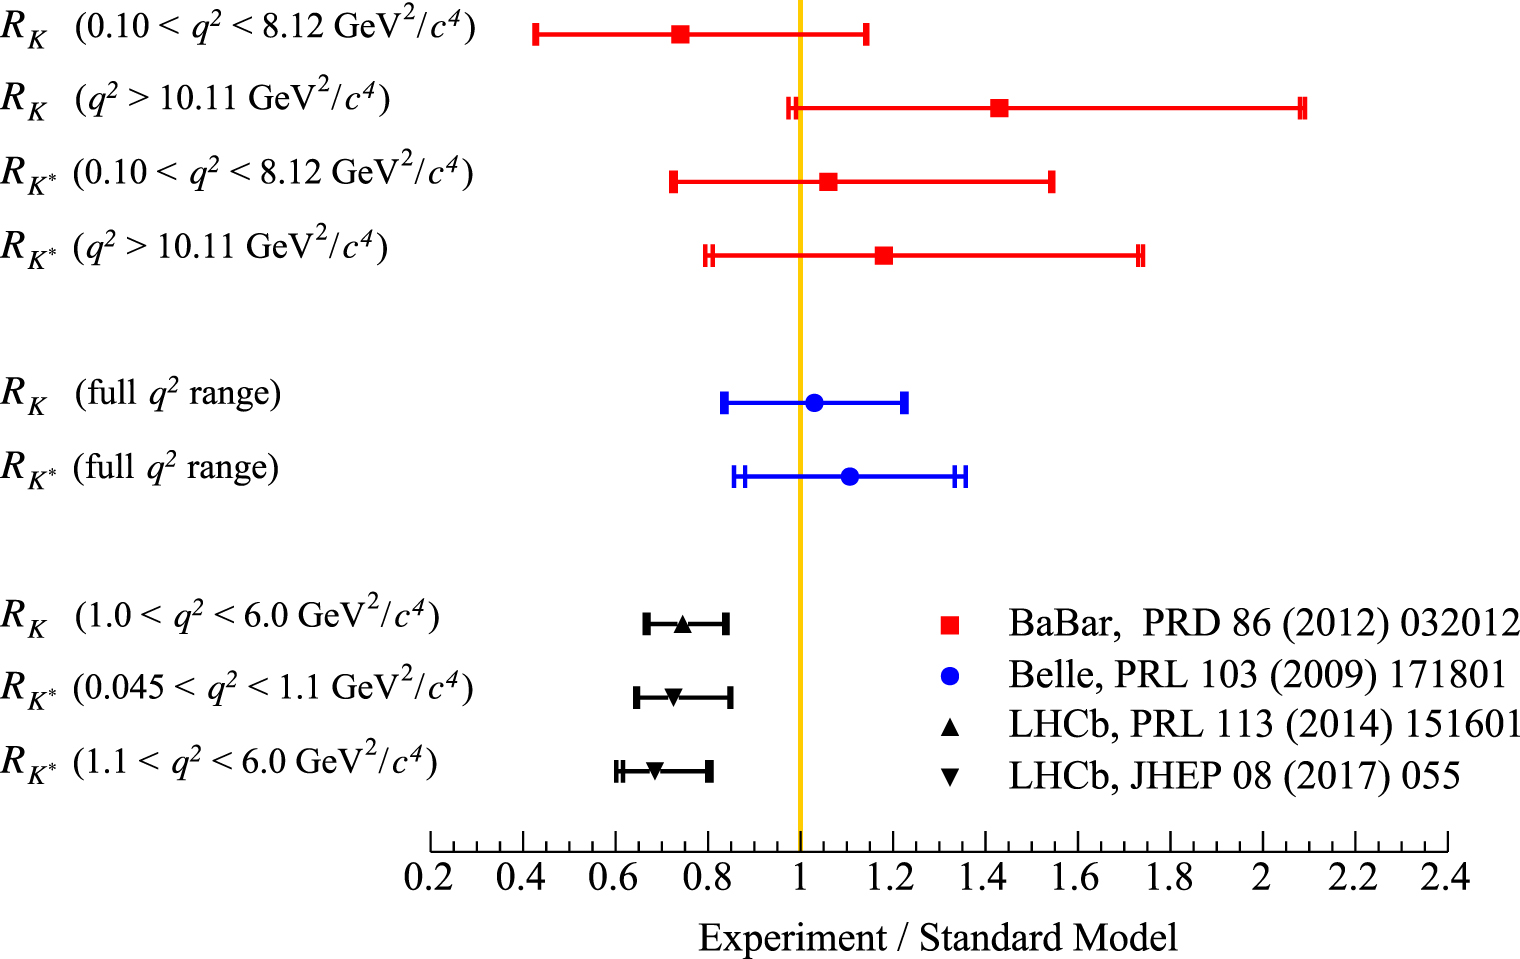
\includegraphics[width=0.75\textwidth]{figures/rkall.jpg}
 	\singlespace
 	\caption{Summary of the ${R}_{{K}^{(*)}}$ measurements performed at the $B$-factories and by the LHCb experiment. Results are presented using different colored markers. The (yellow) vertical line corresponds to the SM prediction. Reprinted from \cite{Bifani_2018}}
 	\label{fig:rkratio}
 \end{figure}


\subsection{$b\rightarrow s$ quark transitions}
As we have seen from the previous section, over the last few years, many observables related to the flavour-changing neutral-current(FCNC) transitions $b\rightarrow l^{+}l^{-}$ have exhibited important deviations from SM expectations. Therefore, in this section, we will take a closer look at these transitions and their sensitivity to potential new physics.

%This anomaly hints at the posibility that $b\rightarrow s$ quark transitions cannot be understood entirely within the SM framework. 
A $b\rightarrow s$ quark transition is an example of a FCNC process\cite{NatFCNC}. In such process, the $s$ and $b$ quark interact via a quantum-loop transition involving predominantly a $W$ boson and either and up, charm, or top quark as shown in Figure \ref{fig:bmesonpic}.

Within the SM, the lowest order processes that could mediate the $b\rightarrow s$ quark transitions are at least of third order and are suppressed by angular momentum conservation and by the chiral nature of the weak force. This suppression is not necessarily present for new-physics particles and that's what makes the study of this decay of particular interest in probing for physics beyond the SM.

 \begin{figure}[H]
 	\centering
 	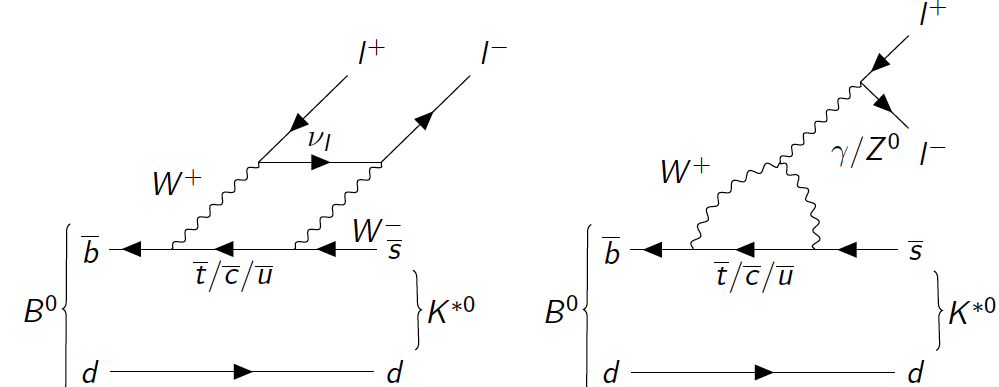
\includegraphics[width=0.95\textwidth]{figures/bmeson.png}
 	\singlespace
 	\caption{Lowest order Feynmann diagrams for $b\rightarrow s$ quark transition.}
 	\label{fig:bmesonpic}
 \end{figure}

\section{The Z'}
There is a multitude of new-physics models that could explain some or all of the $b$ decay anomalies. One example of an extension to the SM that could explain these deviations involves a heavy version of the Z boson, denoted Z'\cite{Buras:2013}. Such an extension to the model must satisfy direct searches for such particles at the CMS\cite{201757}, \cite{Sirunyan:2018exx} and ATLAS \cite{ATLAS-CONF-2016-045} experiments, which in practice means either that the Z' candidate must be at least 30 times heavier than the SM Z boson, or that it must have small couplings to the up and down quarks. If the Z' is very heavy, it would not have a sizable impact on the decay compared with the SM contribution, unless it could change the flavor of quarks directly without going through a quantum-loop transition.

A generic framework of a minimal extension to the SM which explains B anomalies has been introduced in \cite{Dalchenko:2017shg} and we collect here only those formulae of that paper that are essential for our study. The new physics contribution to rare B decays can be described by the following effective Lagrangian 

\begin{equation}
\label{dbscont}
\mathcal{L} \supset \frac{4G_{F}}{\sqrt{2}}V_{tb}V_{ts}^{*}\frac{e^{2}}{16\Pi^{2}}C_{9}O_{9} + h.c.
\end{equation}

where $C_{9}$ is a Wilson coefficient and the effective operator $O_{9}$,

\begin{equation}
O_{9} = (\bar{s}\gamma_{\mu}P_{L}b)(\bar{\mu}\gamma^{\mu}\mu)
\end{equation}

describes a four-fermion interaction, with a left-handed $b-s$ current and a vector current for $\mu$. To fit the current data \cite{PhysRevD.96.055008}, the new physics contribution to $C_{9}$ needs to be $-1.59_{-0.56}^{+0.46}$.

In this model, an extra $U(1)$ gauge group has been introduced, resulting in a new gauge boson, the Z'. This newly introduced particle would have a flavor changing quark coupling $\delta_{bs}$ and a nonuniversal lepton coupling.

Including the contribution from Equation \ref{dbscont}, the dominant terms in the Lagrangian that are allowed by all the existing constraints in order to address the anomalies are then

\begin{equation}
\label{Zlag}
\mathcal{L} \supset Z'_{\mu}[g_{\mu}\bar{\mu}\gamma^{\mu}\mu + g_{\mu}\bar{\nu}_{\mu}\gamma^{\mu}P_{L}\nu_{\mu} + g_{b}\sum_{q=t,b}\bar{q}\gamma^{\mu}P_{L}q (g_{b}\delta_{bs}\bar{s}\gamma^{\mu}P_{L}b +h.c.)]
\end{equation}

The Z' mass is constrained to be less than 5.5(10) TeV in the 1(2)$\sigma$ range to explain the $B$ anomalies\cite{PhysRevD.89.095033}. As the mass gap between the Z' and the SM Z becomes smaller, interference problems start to arise and becomes harder to probe at the LHC. Therefore, for this analysis the lower bound in the search is 250 GeV.

\subsection{4b Bottom Fermion Fusion}

As we can conclude from Equation \ref{Zlag}, the Z' does not significantly couple to first or second generation quarks, which could explain why it has not been observed experimentally yet. However, the Z' can be produced through its couplings to $b$ quarks originating either from sea quarks, or gluon-splitting. 

Therefore, the Z' is associated either with two,one, or no $b$-jets depending on the number of quarks from gluon splitting. The Z' can decay into pairs of $b$ quarks, muons, muon neutrinos, and, if kinematically allowed, top quarks. 

The relevant final states at the LHC are dimuon or di-$b$ resonances. The cross sections behave as follows:

\begin{equation}
\label{crossmu}
\sigma(pp\rightarrow Z' \rightarrow \mu\mu)\propto2g_{b}^{2}(1+k\delta_{bs}^{2})g_{\mu}^{2}
\end{equation}

\begin{equation}
\label{crossb}
\sigma(pp\rightarrow Z' \rightarrow b\bar{b})\propto3g_{b}^{4}(1+k\delta_{bs}^{2})
\end{equation}

where $\delta_{bs}$ regulates the possible production of Z' through b-s quark fusion, and where $k$ contains the $s$-quark PDF contributions. 

For this analysis, the special case when the Z' is associated with two $b$-jets coming from gluon splitting (a process we will refer to as Bottom Fermion fusion (BFF) (see Figure \ref{fig:bff}))and has a di-$b$ jet final state is considered.

 \begin{figure}[h]
 	\centering
 	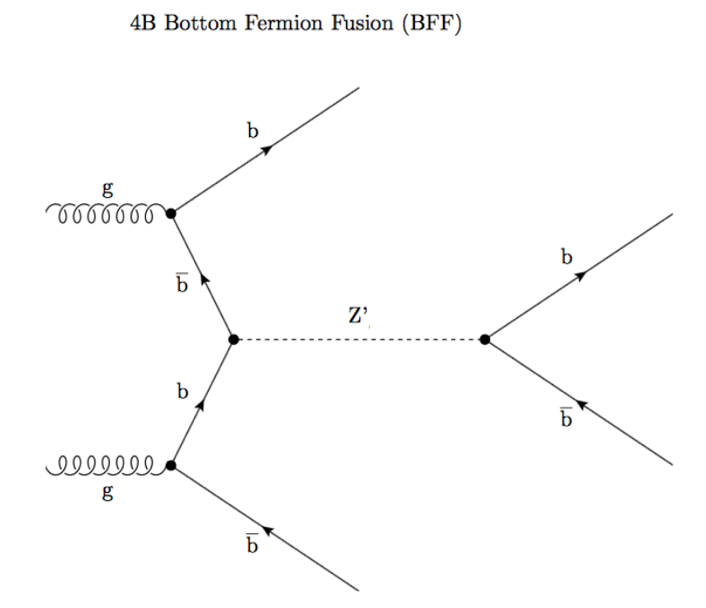
\includegraphics[width=0.5\textwidth]{figures/bff.png}
 	\singlespace
 	\caption{Feynman diagram for bottom fermion fusion (BFF).}
 	\label{fig:bff}
 \end{figure}


%In our case, a possible explanation to the B-decay anomalies could postulate the existence of a new heavy neutral gauge boson, the Z'. Such a particle would couple to $b-s$ quarks and non-universally to leptons. In addition, it would be assumed to couple mostly to third generation quarks to explain why it has not been seen yet by any experiment.
%Basic properties/ Feynman diagram
\subsection{Flavour-violating coupling $\delta_{bs}$}

\begin{figure}[h]
 	\centering
 	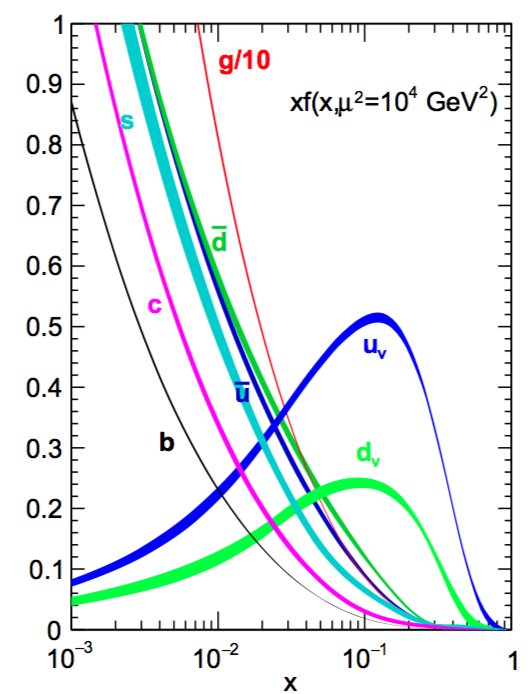
\includegraphics[width=0.6\textwidth]{figures/pdfs.png}
 	\singlespace
 	\caption{PDF for the LHC Run II. Reprinted from \cite{Ball:2014uwa}.}
 	\label{fig:pdfs1}
 \end{figure}

In order to provide an explanation for B-decay anomalies, we need to consider the flavour-violating coupling $\delta_{bs}$. Allowing the Z' boson to couple to $s$ quarks in addition to $b$ quarks results in two times more ways to produce the Z' and two times more ways for it to decay. A non-zero $\delta_{bs}$ will allow the Z's to be produced by $b$ and $\bar{s}$ quarks (in addition to $b\bar{b}$ ones) and this significantly enhances the production cross section since the PDF for the $s$ quark is significantly higher than that for the $b$ quark at the LHC, as we can see from Figure \ref{fig:pdfs1}.

Also, we can see from Equation \ref{crossb} and \ref{crossmu} that when $\delta_{bs}$ goes to zero, the flavor conserving contribution dominates the production of Z'. Likewise, when $\delta_{bs}$ is large but still satisfies the $B$ anomalies (so smaller $g_{b}$) the flavour violating contribution dominates.

%Finally, these effects will also have an impact on our event yields since the analysis strategy is based on the number of $b$-jets we can tage. For example, consider the case when $\delta_{bs}=1$, this implies an equal chance of Z' decaying into a $b-s$ or $b-$ quark pair. As a result, we have at least one less $b$-jet to tag in $75\%$ of all events. An enhanced production cross section due to initial states containing $s$-quarks also translates to a smaller probability of observing processes with diagrams like BFF. This is due to the fact that the $b$-quark PDF contribution is significantly lower than the $s$-quark contribution.

%In conclusion, the impact of $\delta_{bs}$ is to reduce the number of $b$-quark jets that we can expect on the signal. As a result, our acceptance will go down proportionally to $\delta_{bs}$, although our signal cross section rises in turn.

%\subsection{Lifetime calculation}

